\documentclass[10pt,a4paper,parskip=half]{scrartcl}
\usepackage[utf8]{inputenc}
\usepackage[ngerman]{babel}
\usepackage[T1]{fontenc}
\usepackage{graphicx}
\usepackage{setspace}
\usepackage{enumitem}

\usepackage{geometry}
\geometry{a4paper,left=25mm,right=25mm,top=25mm,bottom=45mm}
\usepackage[
automark, % Kapitelangaben in Kopfzeile automatisch erstellen
headsepline, % Trennlinie unter Kopfzeile
ilines % Trennlinie linksbündig ausrichten
]{scrlayer-scrpage }

\useshorthands{+}
\defineshorthand{+S}{\Sentence\ignorespaces}
\defineshorthand{+.}{. \Sentence\ignorespaces}

\pagestyle{scrheadings}
\clearpairofpagestyles

% Kopfzeile
\renewcommand{\headfont}{\normalfont} % Schriftform der Kopfzeile
\ihead{Beitragsordnung des Luftsportverein Degerfeld e.V.\\\textit{\headmark}}
\chead{\\[1ex]\scriptsize{XX XXXXXXX XXXX}}
\ohead{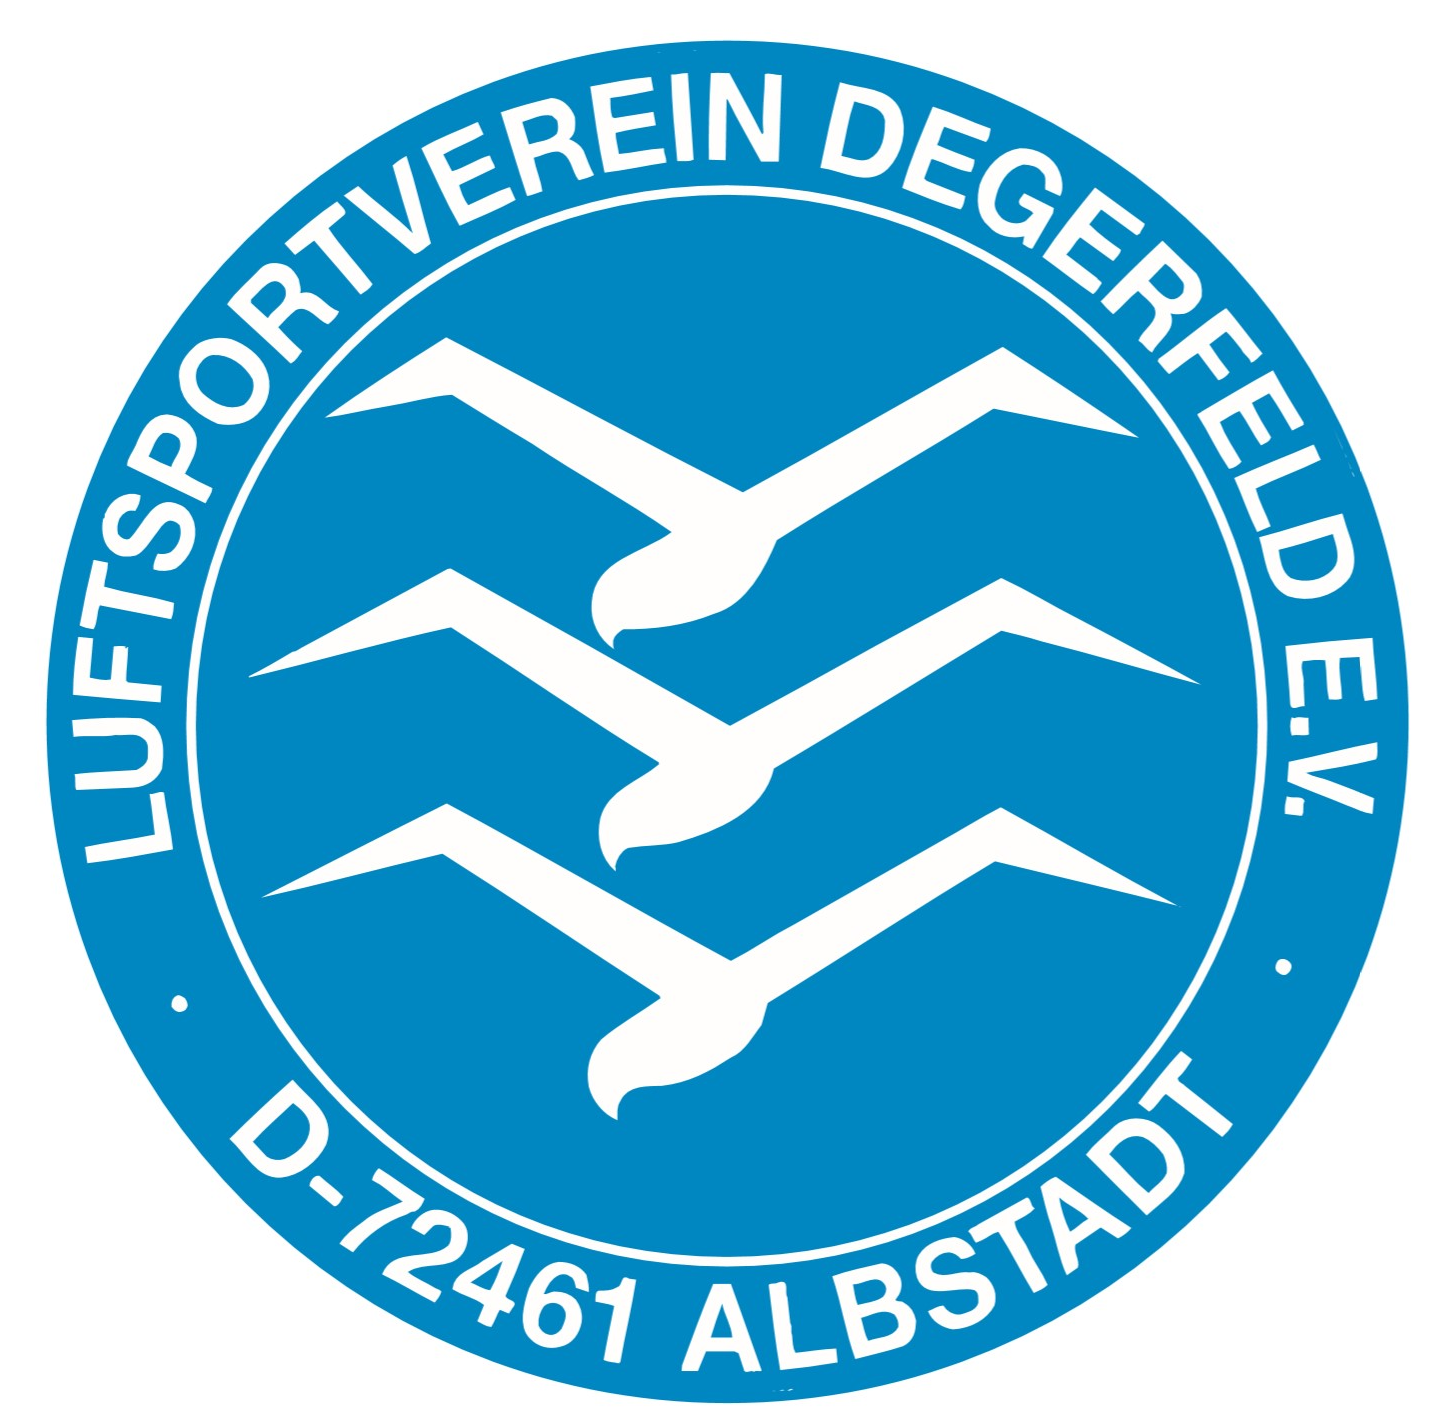
\includegraphics[scale=0.075]{../Logo.png}}
\setlength{\headheight}{20mm} % Höhe der Kopfzeile

% Fußzeile
\ifoot{\today}
\cfoot{}
\ofoot{\pagemark}
\setlength{\footskip}{20mm}

\frenchspacing % erzeugt ein wenig mehr Platz hinter einem Punkt
% Schusterjungen und Hurenkinder vermeiden
\clubpenalty = 10000
\widowpenalty = 10000
\displaywidowpenalty = 10000
\linespread{1.25} % Mehr Zeilenabstand

\usepackage{scrjura,multicol}
\setlength\columnsep{20pt} % Abstand zwischen den Spalten

\usepackage{helvet}
\addtokomafont{disposition}{\rmfamily} 
\addtokomafont{contract.Clause}{\rmfamily}
\renewcommand{\rmdefault}{phv}

\usepackage[hidelinks]{hyperref}


\title{Beitragsordnung des Luftsportverein Degerfeld e.V.}
\subtitle{beschlossen am XX XXXXXX XXXX}

\begin{document}

\thispagestyle{plain}
\begin{center}
  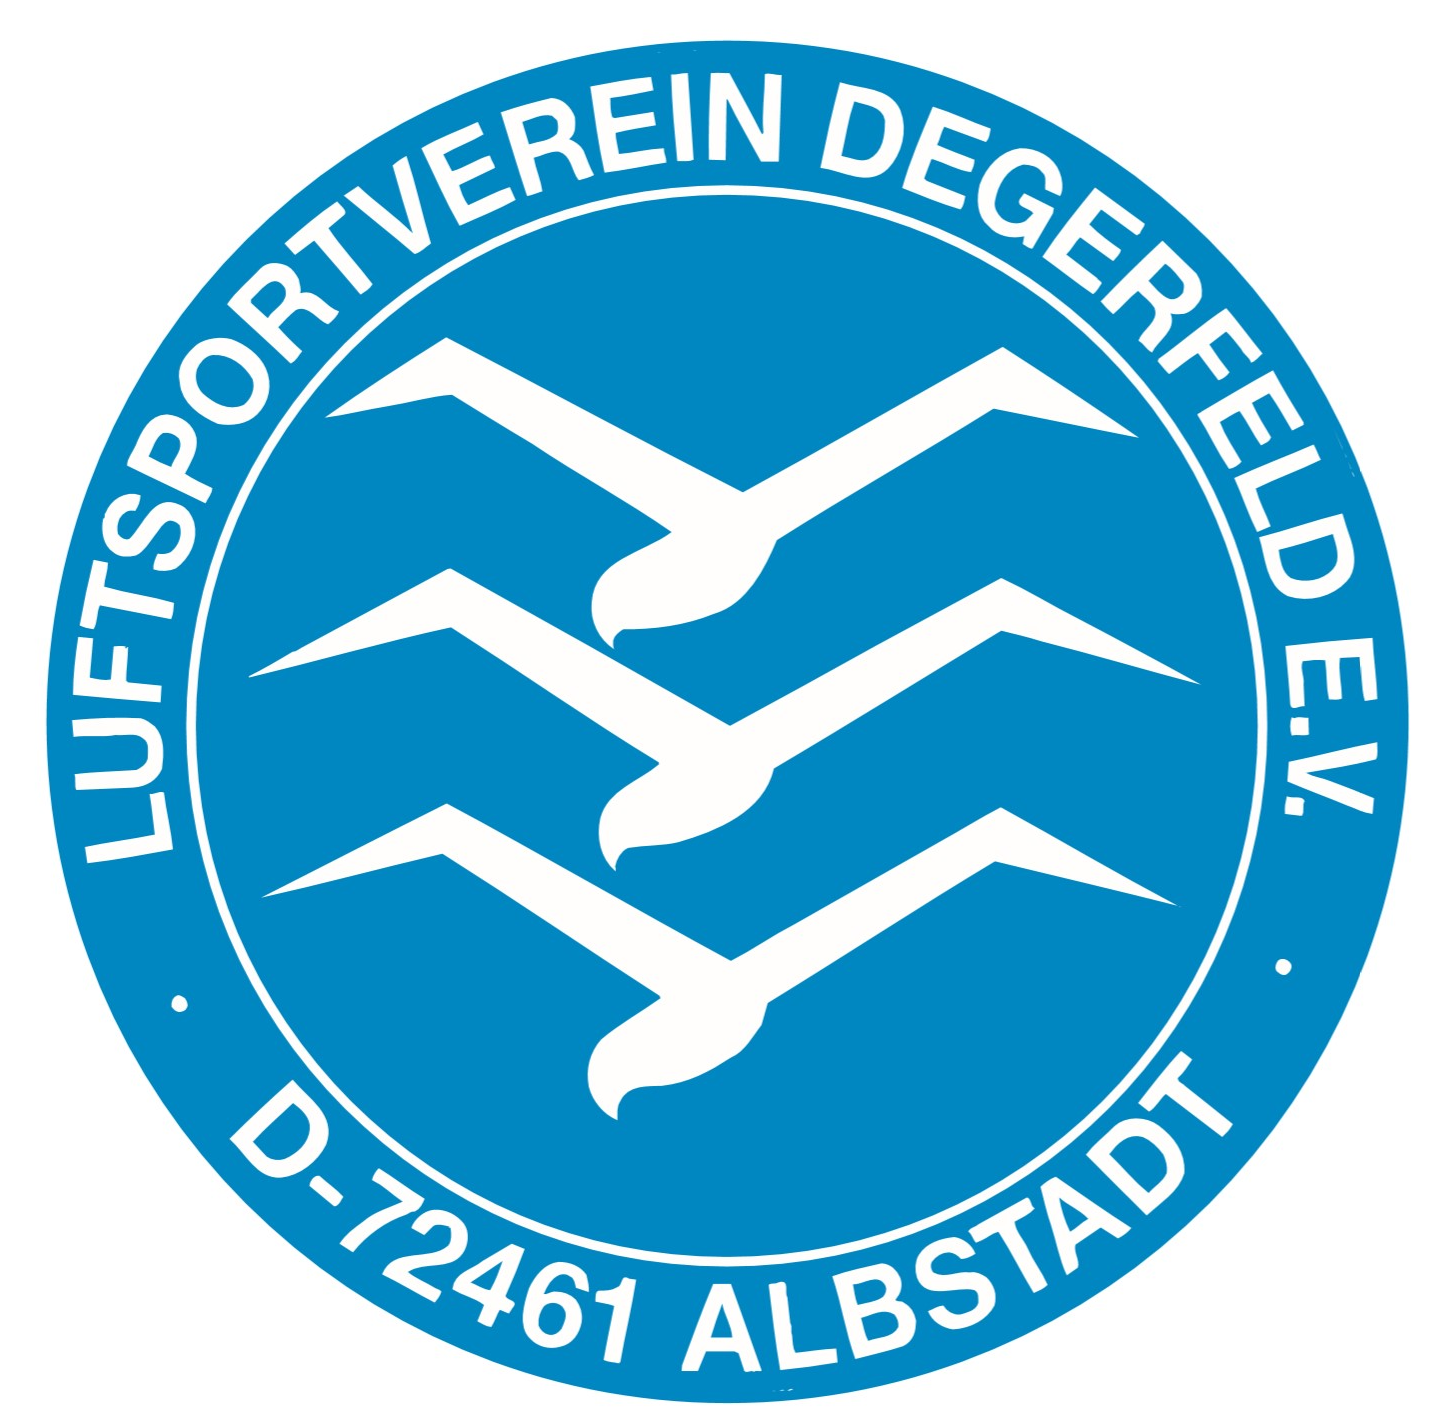
\includegraphics[scale=0.2]{../Logo.png}\\[5ex]
  
  \Huge{\textbf{Beitragsordnung}}\\[1.5ex]
  \large{beschlossen am}\\[1.5ex]
  
  \normalsize
  
  \textbf{\Large{XX XXXXXX XXXX}}\\
  
\end{center}

\begin{contract}
  % \begin{multicols}{2}
    
    \Clause{title={Bezeichnung und Zugehörigkeit}}
    Der Luftsportverein Degerfeld unterhält in ihrem Rahmen eine Jugendgruppe unter dem Namen Luftsportjugend Degerfeld. Die Vereinsjugendgruppe ist dem Jugendverband des baden-württembergischen Luftfahrtverbandes (BWLV) angegliedert.
    
    Die Luftsportjugend wird freiwillig von allen Jugendlichen (Jugendliche Mitglieder sind Jugendliche im Sinne der Definition der Satzung des Vereins) gebildet, die Mitglied des Vereins und des BWLV sind.
    
    Die Beitragsordnung ist eine Ergänzung zur Satzung des Luftsportverein Degerfeld. Die Bezirksjugendordnung und die Jugendordnung des BWLV bilden die Grundlage zur Beitragsordnung.

    \Clause{title={Arbeitsstunden}}
    \subsection*{Grundsätzliche Regelung}


% \end{multicols}
\end{contract}
Jugendordnung beschlossen am 25.03.2023 durch den Ausschuss am xx.04.2023 verabschiedet.

\end{document}